\chapter{State of the Art}
\label{cha:stateOfTheArt}
% The following works propose state-of-the-art methods to get the localization of surgical instruments during MIS.
% feature map -> used in State of the Art. search here and reference to bg
The following works propose current state-of-the-art solutions for surgical instrument segmentation and localization in endoscopic videos.

% better description of this paper / abbreviations of submitted CNNs / teams
% explain better difference between merged method and "single" method

%%%%%%%%% Comparative evaluation of instrument segmentation and tracking methods in minimally invasive surgery %%%%%%%%%
 
Bodenstedt et al.~\cite{miccai15_results2018bodenstedt} present the results of the methods submitted for EndoVis15 (see section~\ref{sec:endovis15}). Additionally, they propose merged results from the submitted models because it significantly increases accuracy in comparison to the best submitted stand-alone method. These results show that the CNN-based methods reached the highest performance compared to other methods. Therefore, in the following part of this chapter, only CNN-based methods concerning image-based segmentation of surgical instruments will be described.
% SEG-KIT-CNN
For EndoVis15-S, SEG-KIT-CNN is proposed: It is a FCN that uses VGG-16~\cite{simonyan2014vgg} as an encoder.

%%%%%%%%% Real-Time Segmentation of Non-rigid Surgical Tools Based on Deep Learning and Tracking %%%%%%%%%
Garcia et al.~\cite{garcia2017segm_nonrigid_book} propose two adapted FCNs for EndoVis15-S: FCN and FCN-real-time.
The forward evaluation takes 100ms for the FCN which is below the frame rate of an endoscopic video. The frame rate of an endoscopic video is usually 25 frames per second (fps), 30~fps or 60~fps.
% explanation not soo good
The FCN-real-time approach overcomes this problem by estimating an affine transformation on the instrument between the time of two segmentations of the network. 
When a frame is read from the surgical video feed, it is sent to the FCN-real-time only if the network is not busy processing the previous frame.

%%%%%%%%% Deep Residual Learning for Instrument Segmentation on Robotic Surgery %%%%%%%%%
Pakhmov et al.~\cite{deep_residual_instr_segm2017pakhmov} propose a ResNet-101 which is converted into a FCN for EndoVis15-S (ResNet-FCN).

%%%%%%%%% Surgical tool segmentation using a hybrid deep CNN-RNN auto encoder-decoder %%%%%%%%%
% in picture of network: take rigid set but results are for robotic ?? ok.
% include ref for recurrent network!
Attia et al.~\cite{Attia2017_surg_tool_cnn-rnn} provide a Convolutional Neural Network - Recurrent Neural Network (hybrid CNN-RNN) auto encoder-decoder network~(see figure~\ref{img:hybrid_cnn_rnn}) for instrument segmentation for EndoVis15-S.

\begin{figure}
	\centering
	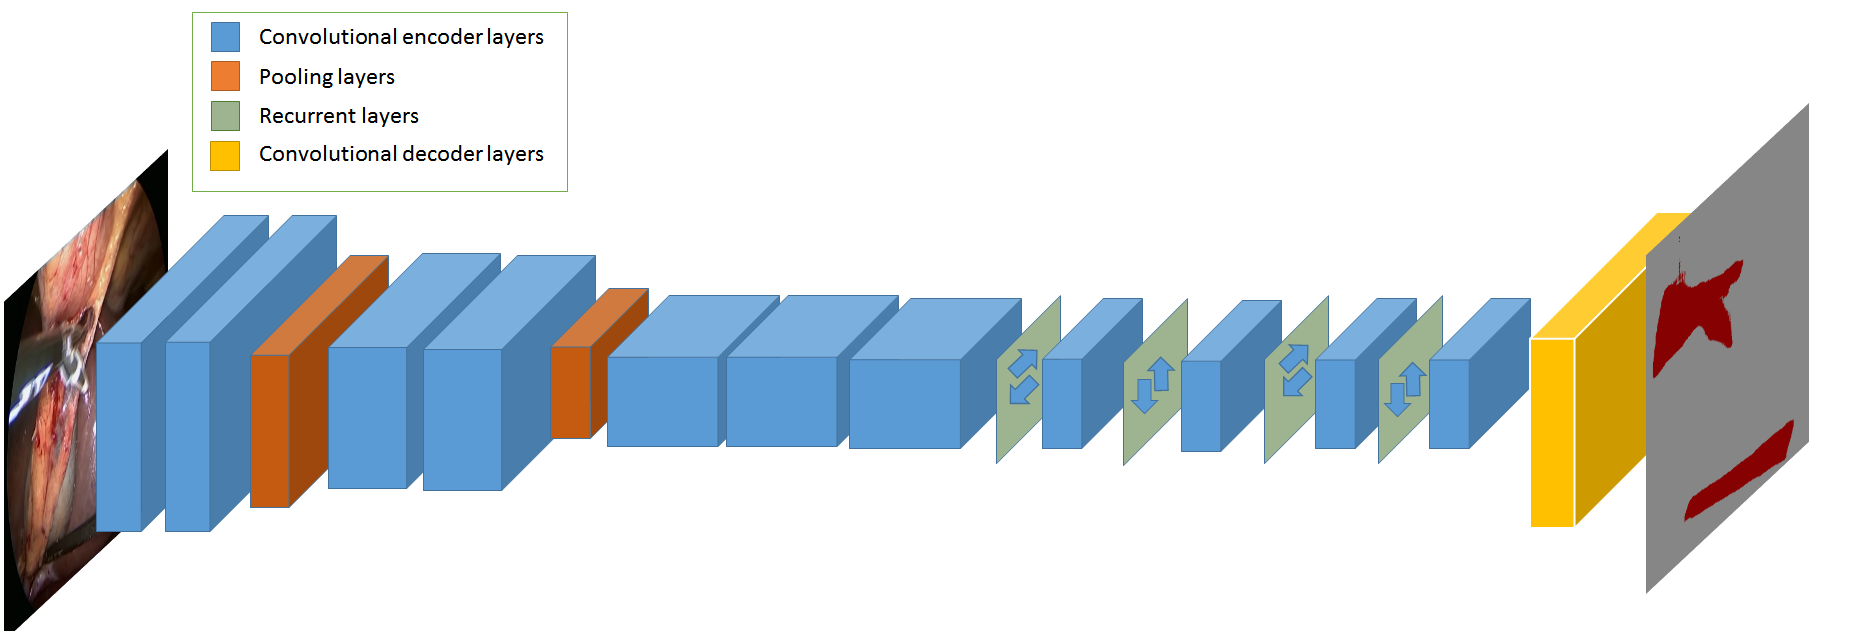
\includegraphics[width=.8\textwidth]{images/networks/hybrid_cnn_rnn.png}
	\caption[CNN-RNN architecture~\cite{Attia2017_surg_tool_cnn-rnn}]{Proposed hybrid CNN-RNN architecture by Attia et al.~\cite{Attia2017_surg_tool_cnn-rnn}.
	The encoder phase of the network consists of seven convolutional layers denoted as blue blocks, 
	the two max-pooling layers are denoted as orange blocks. 
	The feature maps extracted by the encoder part of the network are fed into 4 layers of the recurrent network, denoted as green masks
	with 4 decoupled directions. The output mask of the instrument is reconstructed using an auto decoder network, denoted with yellow blocks.}
	\label{img:hybrid_cnn_rnn}
\end{figure}

%%%%%%%%% Concurrent Segmentation and Localization for Tracking of Surgical Instruments %%%%%%%%%
Laina et al.~\cite{Laina2017} propose three different CNN-based approaches to predict the location of surgical instruments (see figure~\ref{img:csl_network}).
They are abbreviated as L-network, SL-network and CSL-network. 
All of the proposed networks share ResNet-50~\cite{deep_res_learning_img_rec2016He} as encoder part.

The decoder part of the L-network regresses the positions of the instrument directly as a 2x$n_i$ dimensional vector, where $n_i$ is one predicted location of one instrument. This method is frequently used in literature.~\cite{landmark_localization_2Dvector2016rupprecht}
The segmentation task of the instrument is excluded in this approach.

In the SL-network, the prediction of the 2D locations of the instrument and the segmentation of the instrument are combined in one architecture. 
Both tasks share weights along the encoder part and split into two distinct parts at the decoder part of the network. The prediction of the instrument positions is solved like in the L-model.
For the segmentation task, the probability of each pixel of belonging to the instrument or the background is predicted.

The CSL-network predicts the position of the instrument by regressing a heatmap instead of the exact coordinates.
The heatmap for training is created by applying a two-dimensional Gaussian function to the ground truth position of the instrument (see section~\ref{sec:heatmaps}). 
By applying this method, the problem that ground truth annotations of the instrument position
can differ by several pixels is avoided. The segmentation and localization task share weights over the entire network because the heatmaps have the same size as the segmentation masks.
The CSL-network outperforms the two other proposed methods.

\begin{figure}
	\centering
	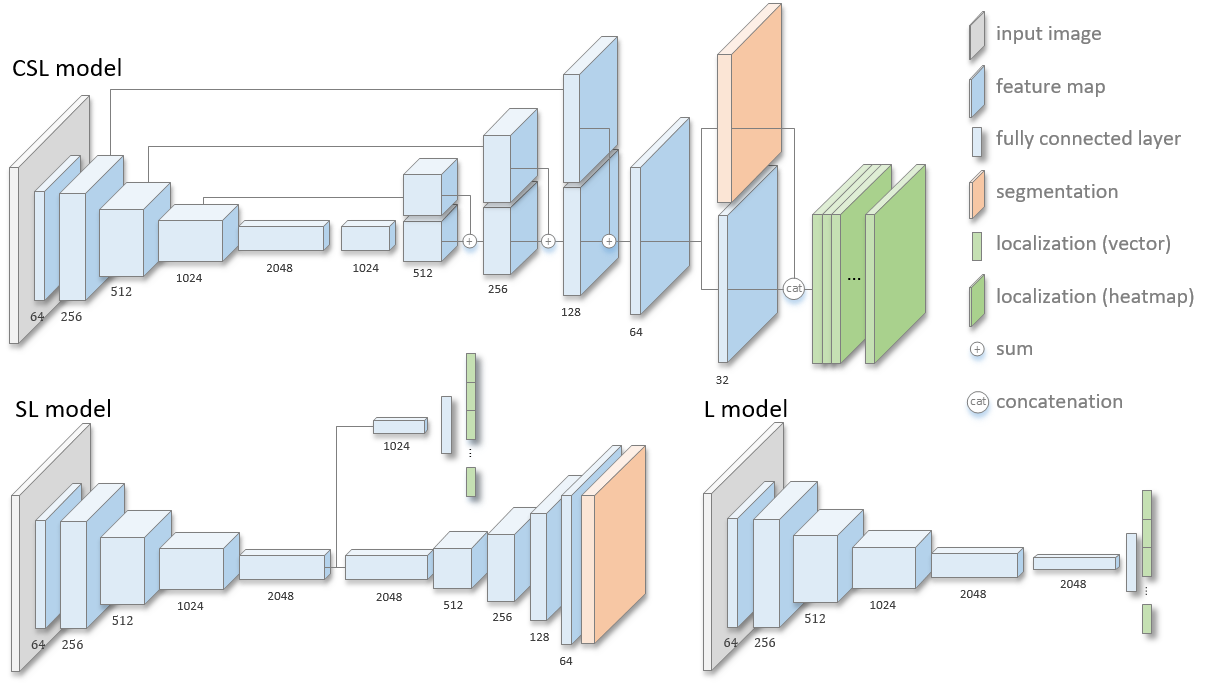
\includegraphics[width=.6\textwidth]{images/networks/CSL_network.png}
	\caption[Concurrent Segmentation and Tracking Networks~\cite{Laina2017}]{The three proposed network architektures in Laina et al.~\cite{Laina2017}}
	\label{img:csl_network}
\end{figure}

%%%%%%%%% Articulated Multi-Instrument 2-D Pose Estimation Using Fully Convolutional Networks %%%%%%%%%%%
% too complicated maybe
Du et al.~\cite{du2018_2D_pose_est_CNN} solved the localization task by using a fully convolutional detection-regression network (FCN-det-reg) (see figure~\ref{detection-regression-net}), where the instrument joints and associations between joint pairs are located by the detection subnetwork and subsequently redefined by the regression subnetwork. 

\begin{figure}
	\centering
	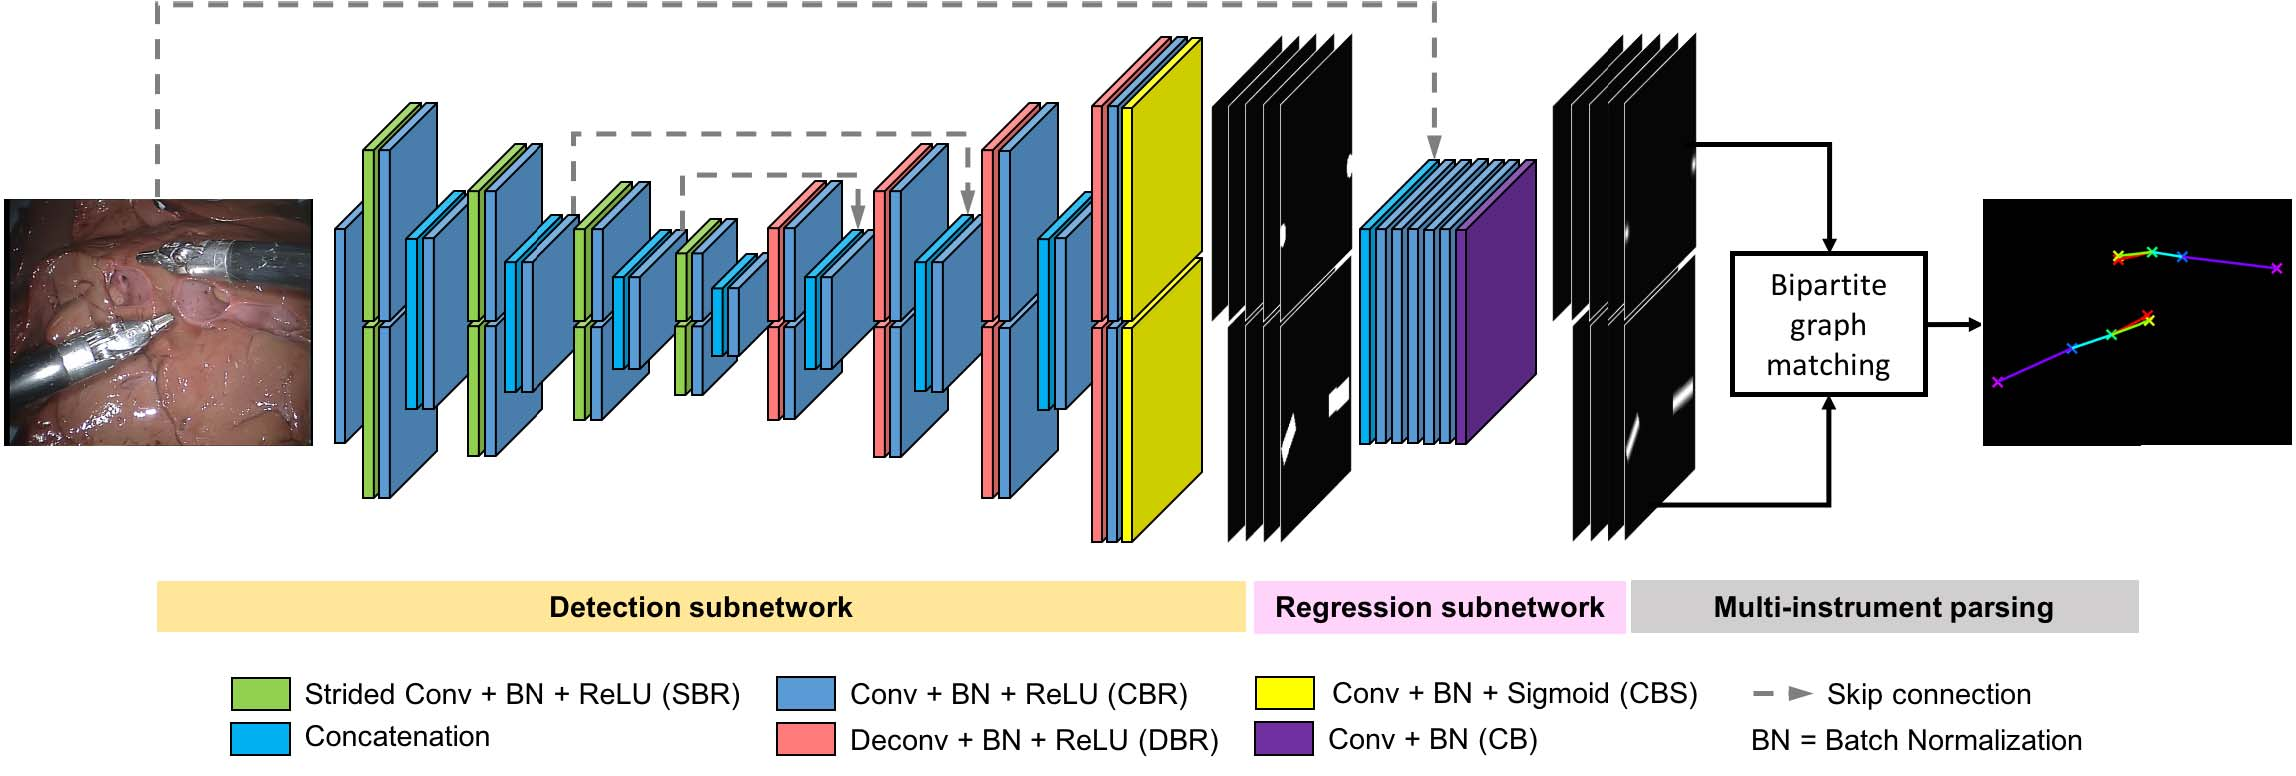
\includegraphics[width=.8\textwidth]{images/networks/detection-regression.jpg}
 	\caption[Detection-regression network~\cite{du2018_2D_pose_est_CNN}]{Structure of the detection-regression network proposed in Du et al.~\cite{du2018_2D_pose_est_CNN}}
 	\label{detection-regression-net}
\end{figure}

Positions of the surgical instruments are inferred using maximum bipartite graph matching~\cite{bipartite_graph2005schwartz}.
The EndoVis15-T (see section~\ref{sec:endovis15}) ground truth annotations were modified and replaced by self-generated annotations (see figure~\ref{modified_gt_2D_pose}).

\begin{figure}
\centering
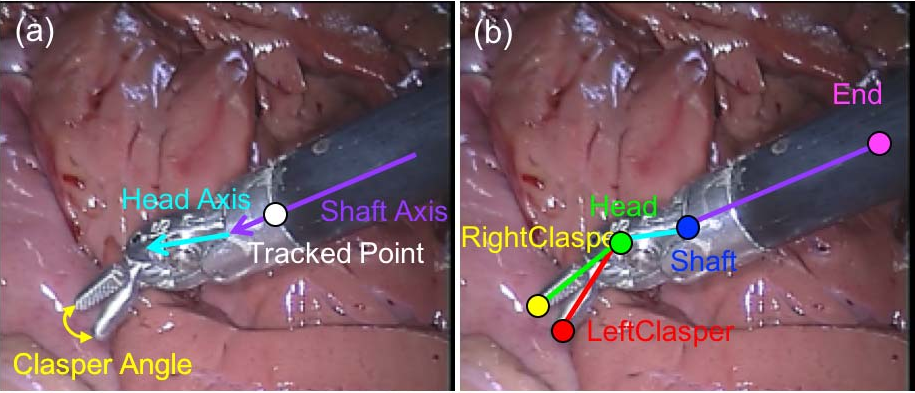
\includegraphics[width=.6\textwidth]{images/dataset/annotated_gt.png}
\caption[Modified ground truth annotation~\cite{du2018_2D_pose_est_CNN}]{The original (a) and modified (b) ground truth annotations for EndoVis15-T.}
\label{modified_gt_2D_pose}
\end{figure}

The detection part of the network (see figure~\ref{detection-regression-net}) consists of two branches. 
The first branch is used to predict probability maps for each joint of the surgical instrument, 
the second branch is used to predict association probability maps for each joint pair.
% Therefore, the ground truth for the detection subnetwork is constructed as a set of the joint and joint pair binary maps (see figure~\ref{img:gt_association_binary_joint}). -> unnecessary, delete pic
From the prediction of the detection part, a coarse position of the instrument is obtained. With the regression part of the network, that takes the prediction of the detection part as an input, refined positions of the joints are obtained.
The ground truth for the regression subnetwork for each instrument joint location consists of heatmaps formed by a two-dimensional Gaussian distribution at the labeled position of the joint. 
The ground truth for the association between joint pairs are formed by a Gaussian distribution along the joint pair center line.
The approach to use heatmaps in form of images to predict the instrument position is similar to Laina et al.~\cite{Laina2017}.

Notably, it is not possible to compare the FCN-det-reg results directly to the other results: The provided ground truth is modified, the results that exceed a certain threshold are excluded from evaluation, and the training procedure is different from the challenge guidelines.

% Notably, the network is trained with the entire training data instead of a LOSO training strategy as specified by the EndoVis15 challenge guidelines (see section~\ref{sec:endovis15_robotic_test}). 
% That makes the results incomparable to the results that are obtained by other solutions trained accordingly to the challenge guidelines.

%%%%%%%%%%  Simultaneous Recognition and Pose Estimation of Instruments in Minimally Invasive Surgery %%%%%%%%% 
%Kurmann et al.~\cite{kurmann2017sim_recogn_pose_estim} propose a modified U-Net architecture (see figure~\ref{img:kurmann_u_net_multi_instr}) to detect multiple instrument positions.
%The results are calculated
%
%\begin{figure}
%	\centering
%	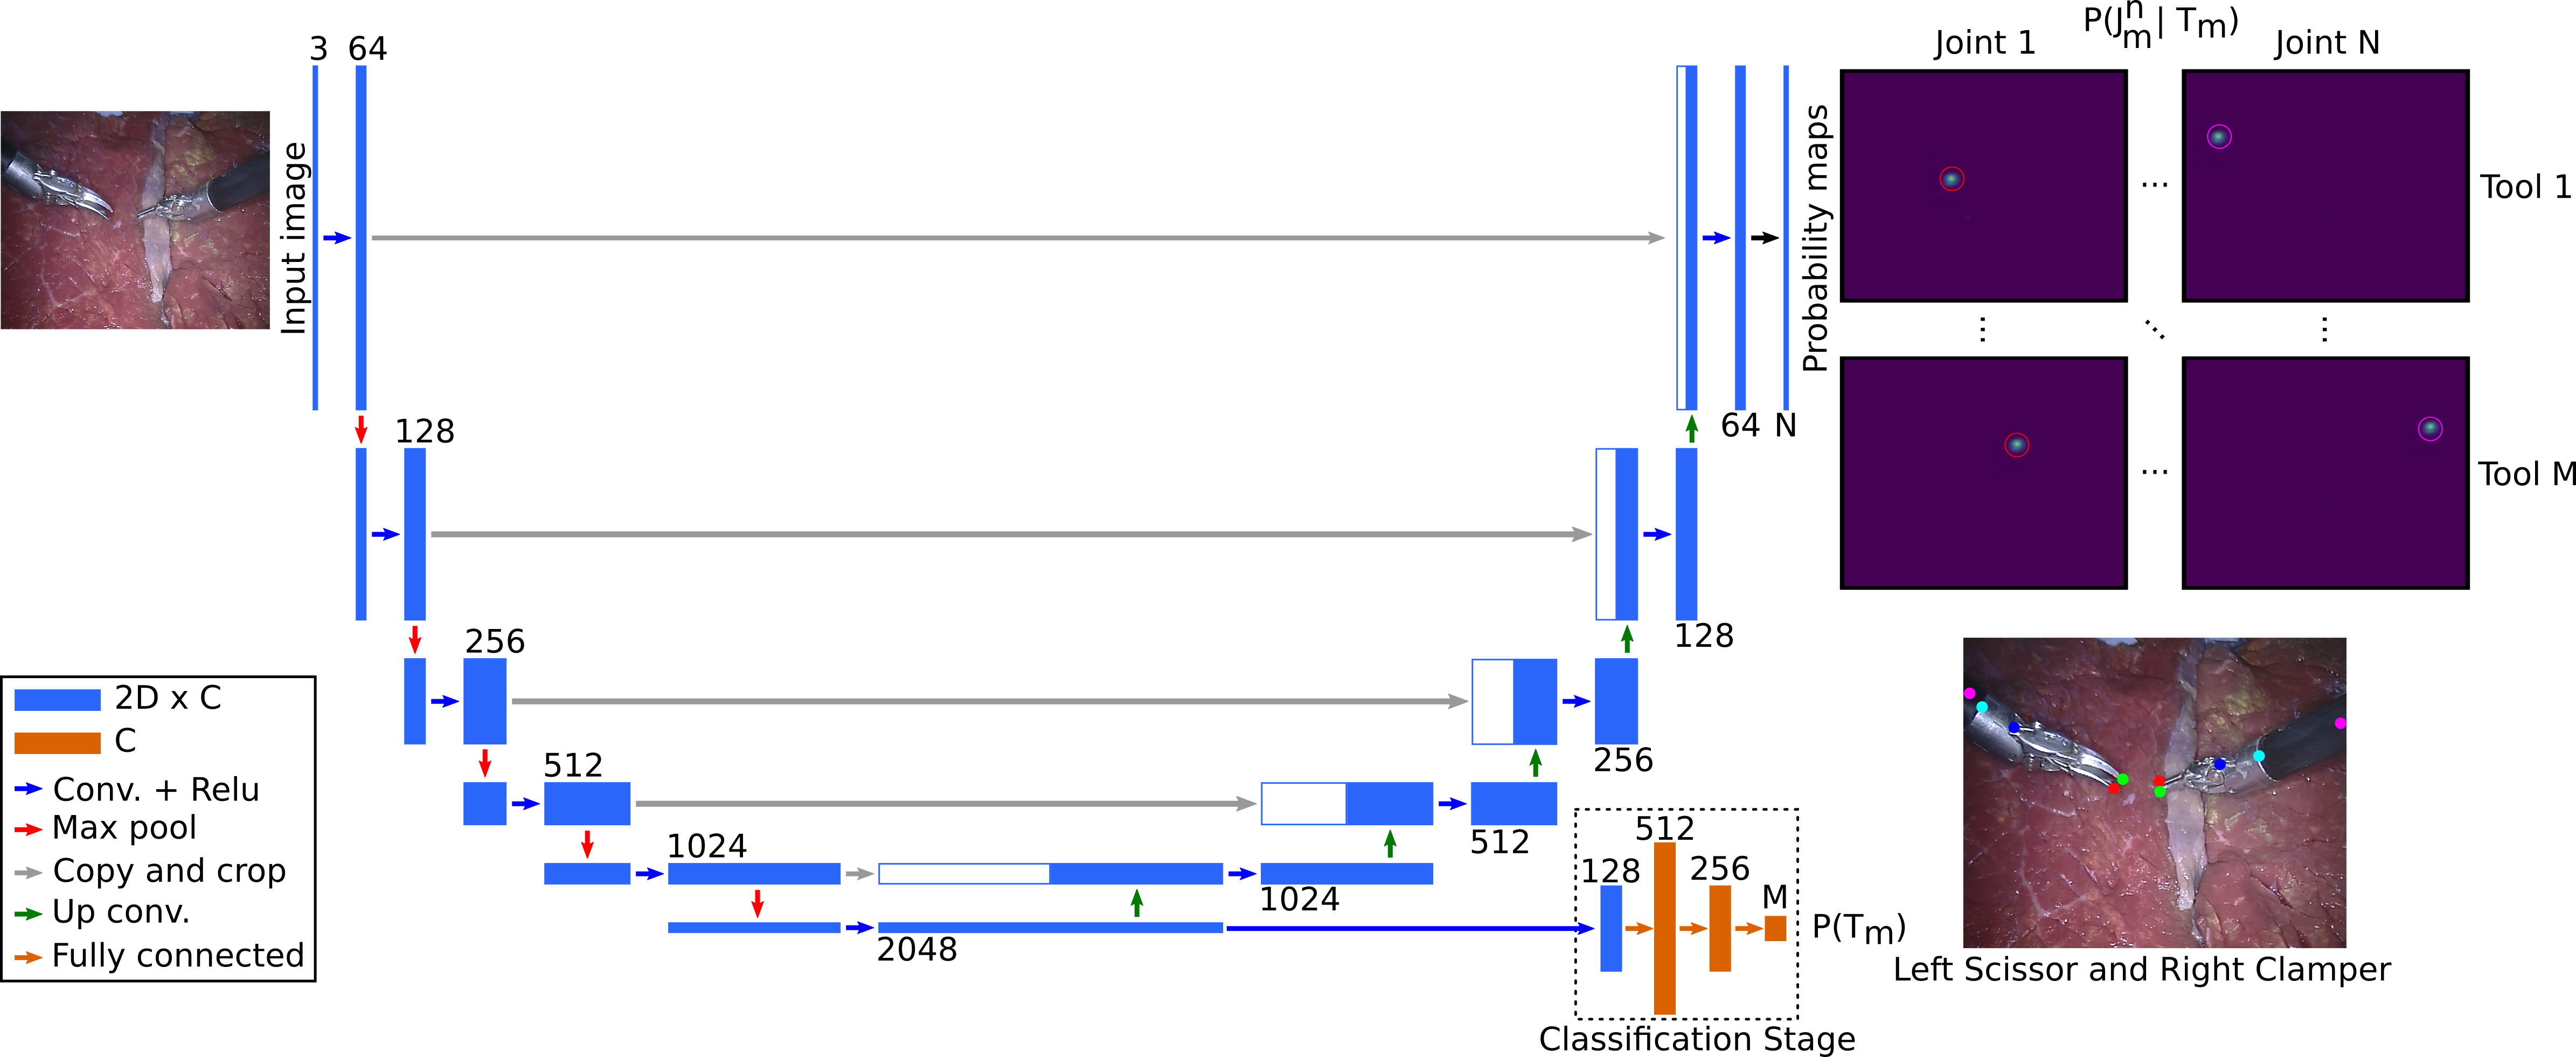
\includegraphics[width=.7\textwidth]{images/networks/multi_instr_u-net.png}
%	\caption{U-Net based multi-instrument detector network architecture proposed by Kurmann et al.~\cite{kurmann2017sim_recogn_pose_estim}}
%	\label{img:kurmann_u_net_multi_instr}
%\end{figure}

%%%%%%%%% Automatic Instrument Segmentation in Robot-Assisted Surgery Using Deep Learning %%%%%%%%%
Shvets et al.~\cite{Shvets2018} used four different networks for EndoVis17-S (see section\ref{sec:endovis17}):
U-Net (see figure~\ref{img:basic_u-net}), TernausNet-11 and TernausNet-16 which are a modifications of U-Net, and one network that is a modification of LinkNet~\cite{linknet2017Chaurasia}.
TernausNet-16~(see also figure~\ref{img:ternausnet16}) outperforms the other networks in the segmentation tasks except for the inference time.
VGG16~\cite{simonyan2014vgg}, pre-trained (see section~\ref{nn:testing}) on ImageNet, is used as encoder  for TernausNet-16.

\begin{figure}
	\centering
	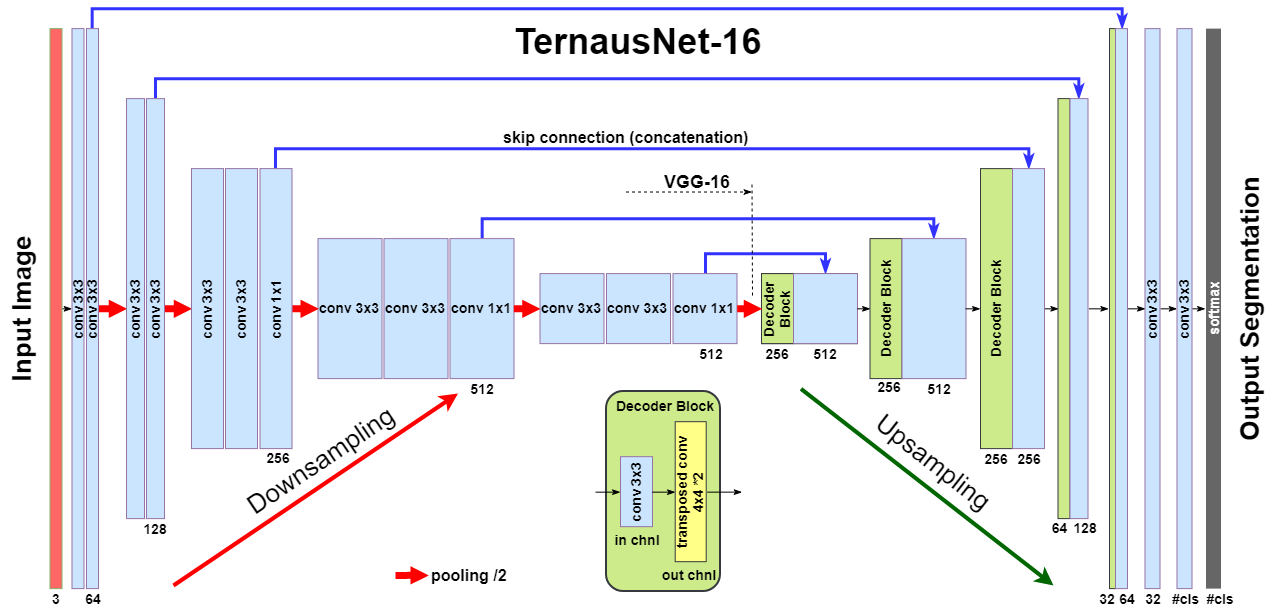
\includegraphics[width=.8\textwidth]{images/networks/TernausNet16.png}
	\caption[TernausNet-16~\cite{Shvets2018}]{Structure of the segmentation network TernausNet-16. 
	Each box corresponds to a multi-channel feature map with the number of channels denoted below the box. 
	The height of each box represents the corresponding feature map resolution. 
	The blue arrows illustrate skip-connections where information is transmitted from the decoder
	to the encoder phase of the network.~\cite{Shvets2018}}
	\label{img:ternausnet16}
\end{figure}

%Localization methods: TRA-KIT, TRA-UGA.
% also: specify localization methods
To solve specifically the localization task of EndoVis15-T, Bodenstedt et al.~\cite{miccai15_results2018bodenstedt} propose two approaches that are not CNN-like: TRA-UGA~\cite{SEG-UGA2016agustinos} and TRA-KIT-RF~\cite{KIT-TRA2016bodenstedt}.

An overview of the previously proposed methods is is given in table~\ref{tab:summary_results_endovis15}

% note: \cite{du2018_2D_pose_est_CNN} doesn't train with challenge guidelines
% Kurmann et al. fehlt!
\begin{table}
\centering
% \small
%\resizebox{!}{1.00cm}{
\begin{tabular}{l c c c c c c c}
\hline\noalign{\smallskip} 
\multicolumn{8}{c}{\textbf{EndoVis15-S results}} \\
 & \multicolumn{2}{r}{b.acc.} accuracy & recall & prec. & spec. & Dice & IoU \\ \hline 
CSL-network~\cite{Laina2017} & 92.6 & - & 86.2 & - & 99.0 &  88.9 & - \\
SEG-KIT-CNN~\cite{KIT-TRA2016bodenstedt} & - &  96 & 77 & 86 & - & 81 & - \\
%network & b.acc. & accuracy & recall/sensitivity & prec. & spec. & Dice & IoU & distance \\
SEG-UGA~\cite{SEG-UGA2016agustinos} & - & 96 & 66 & 95 & - & 78 & - \\
FCN~\cite{garcia2017segm_nonrigid_book} & 83.7 & - & 72.2 & - & 95.2 & - & - \\
FCN-real-time~\cite{garcia2017segm_nonrigid_book} & 88.3 & - & 87.8 & - & 88.7 & - & - \\
ResNet-FCN~\cite{deep_residual_instr_segm2017pakhmov} & 92.3 & - & 85.7 & - & 98.8 & - & - \\
CNN-RNN~\cite{Attia2017_surg_tool_cnn-rnn} & 93.3 & - & 90.4 & - & 96.1 & - & 82.7 \\
\hline 
\end{tabular}
%}
\caption[Results EndoVis15-S, State of the Art]{Results of EndoVis15-S (see section~\ref{sec:endovis15}) for every proposed paper. Balanced accuracy (b.acc.), accuracy, recall, precision~(prec.), specificity (spec.), Dice, Intersection over Union~(IoU) are given in \%. For definition of evaluation metrics see section~\ref{sec:evaluation_metrics}.}
\label{tab:summary_results_endovis15}
\end{table}


% maybe include more from Bodenstedt paper
\begin{table}
\centering
\begin{tabular}{l c c c}
\hline\noalign{\smallskip} 
\multicolumn{4}{c}{\textbf{EndoVis15-T results}} \\
& distance LOSO & distance T4 & distance-total \\ \hline
CSL-network~\cite{Laina2017} & 20.68 & 49.68 & 34.46 \\
TRA-KIT~\cite{KIT-TRA2016bodenstedt} & - & - & 106.6 \\
TRA-UGA~\cite{SEG-UGA2016agustinos} & - & - & 34.9 \\
% TRA-MERGED~\cite{KIT-TRA2016bodenstedt} & - & - & 32.0 \\
%\hline\noalign{\smallskip} 
\shortstack{FCN-det-reg~\cite{du2018_2D_pose_est_CNN} train set\\ \emph{thresh=20px}} & - & - & 3.36 \\
\shortstack{FCN-det-reg~\cite{du2018_2D_pose_est_CNN} test set\\ \emph{thresh=20px}} & - & 6.96 & - \\
\shortstack{FCN-det-reg~\cite{du2018_2D_pose_est_CNN} test set\\ \emph{thresh=30px}} & - & 7.98 & - \\
\end{tabular}
\caption[Results EndoVis15-T, State of the Art]{Results of EndoVis15-T (see section~\ref{sec:endovis15}) for every proposed localization solution. The distance between predicted position of the instrument and labeled ground truth position of the instrument is given in pixels. The evaluations refer to the results for models trained according to LOSO fashion (distance LOSO), the results for models trained with all training sets and tested on the test sets (T4), and to the mean value of the results of both training methods (distance in total).}
\end{table}



%%%% TEST %%%%
%\begin{table}
%\begin{adjustbox}{center=\textwidth}
%\begin{tabular}{l c c c c c}
%\hline\noalign{\smallskip}
% & Dataset1 left/right instr. & Dataset2 & Dataset3 & Dataset4 & mean dist.\\
%\hline\noalign{\smallskip}
%Laina et al. &  $39.0 / 30.8$ & 9.7 & 10.9 & 13.0 & 20.7 \\
%LOC-03 &  $17.58 / 15.15$ & $11.36$ & $10.83 $ & $12.05 $ & $13.85 $\\ [0.5ex] 
%\end{tabular}
%\end{adjustbox}
%\caption{test2}+
%\label{tab:test2}
%\end{table}
%
%\begin{table}
%\begin{tabular}{l c c c}
%\hline\noalign{\smallskip}
% & Dataset5 left/right instr.& Dataset6 left/right instr.& mean dist.\\
% \hline\noalign{\smallskip}
% Laina et al. & 38.4/60.0 & 36.4/63.9 & 49.68\\
%LOC-04 &  $89.80 / 117.91 $ & $ 88.17 / 120.02$ & $106.4 $ \\ [0.5ex]
%\end{tabular}
%\caption{test1}
%\label{tab:test1}
%\end{table}

% \begin{table}
% \centering
% \begin{tabular}{l r}
% \hline\noalign{\smallskip} \\
%  & loc.error  \\ \hline
% Dataset1 &  39.0/30.8\\
% Dataset2 & 9.7\\
% Dataset3 & 10.9\\
% Dataset4 & 13.0 \\
% Dataset5 & 38.4/60.0\\
% Dataset6 & 36.4/63.9\\ \hline
% \hline 
% mean &  24.8/51.6\\ \hline
% \end{tabular}
% \caption{test3}
% \label{tab:test3}
%\end{table}




